\documentclass[9pt]{amsart}
\usepackage{amsmath}
\usepackage{csquotes}
\usepackage{enumitem}
\usepackage{multicol}
\usepackage{caption}
\usepackage[margin=1in]{geometry}
\usepackage{tikz}

\title{FEM By Hand}
\author{Arden Rasmussen}
\date{\today}

\newenvironment{Figure}
{\par\medskip\noindent\minipage{\linewidth}}
{\endminipage\par\medskip}

\newcommand{\hdiv}[3]{
  \vspace{#1}%
  \noindent\rule{\textwidth}{#2}%
  \vspace{#3}%
}

\newcommand{\e}[2]{_{#1}^{(#2)}}
\newcommand{\pder}[2]{\frac{\partial #1}{\partial #2}}


\begin{document}
\maketitle

\hdiv{2pt}{1pt}{2pt}

\begin{figure}[htpb]
  \begin{center}
    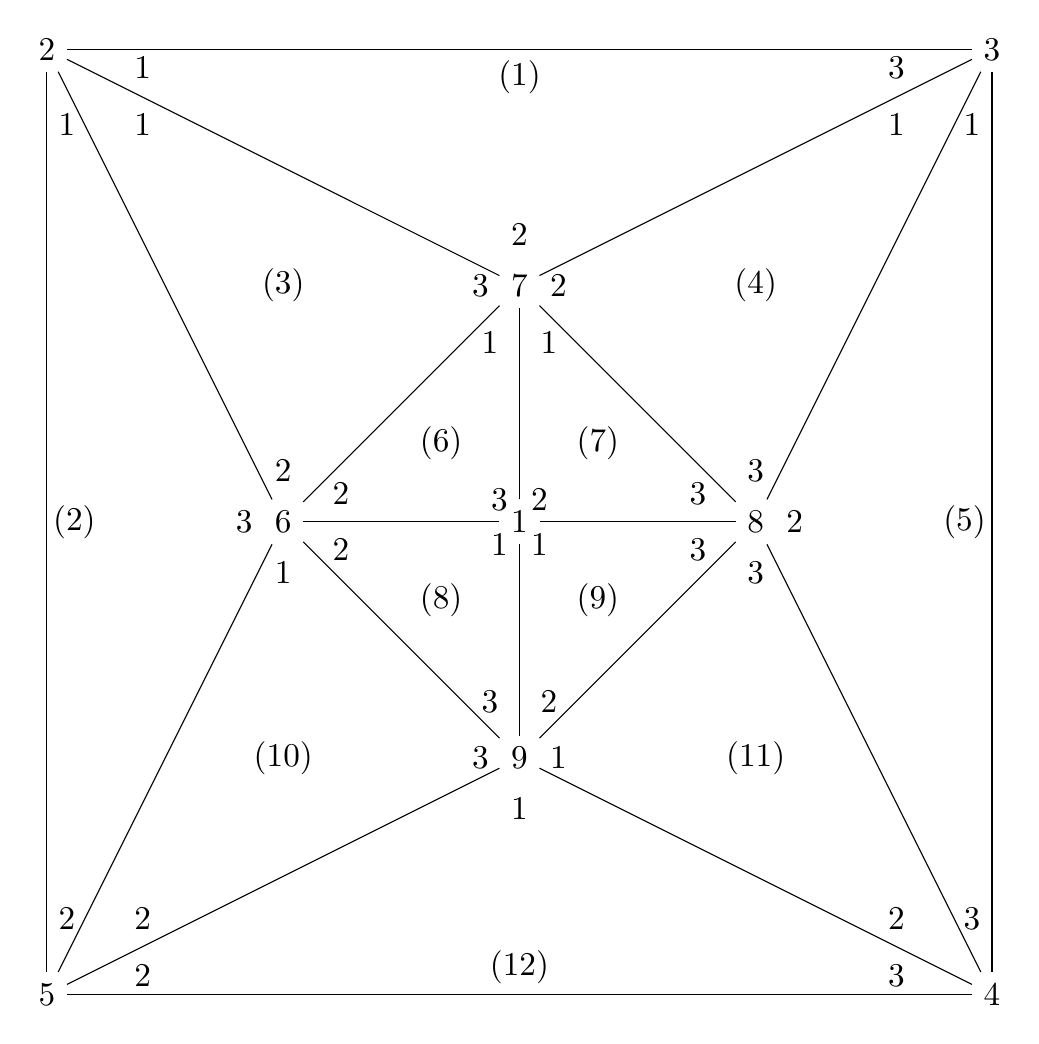
\begin{tikzpicture}[scale=1.2, transform shape]
      \node (a1) at (0,0){1};
      % \coordinate (a1) at (0,0);
      \node (a2) at (-5,5){2};
      \node (a3) at (5,5){3};
      \node (a4) at (5,-5){4};
      \node (a5) at (-5,-5){5};
      \node (a6) at (-2.5,0){6};
      \node (a7) at (0,2.5){7};
      \node (a8) at (2.5,0){8};
      \node (a9) at (0,-2.5){9};

      \node at (a1)[above right]{2};
      \node at (a1)[above left]{3};
      \node at (a1)[below right]{1};
      \node at (a1)[below left]{1};

      \node at (a2)[below=0.8cm,right=0.8cm]{1};
      \node at (a2)[below=0.8cm,right]{1};
      \node at (a2)[below=0.2cm,right=0.8cm]{1};

      \node at (a3)[below=0.8cm,left=0.8cm]{1};
      \node at (a3)[below=0.8cm,left]{1};
      \node at (a3)[below=0.2cm,left=0.8cm]{3};

      \node at (a4)[above=0.8cm,left=0.8cm]{2};
      \node at (a4)[above=0.8cm,left]{3};
      \node at (a4)[above=0.2cm,left=0.8cm]{3};

      \node at (a5)[above=0.8cm,right=0.8cm]{2};
      \node at (a5)[above=0.8cm,right]{2};
      \node at (a5)[above=0.2cm,right=0.8cm]{2};

      \node at (a6)[left=0.2cm]{3};
      \node at (a6)[above=0.3cm]{2};
      \node at (a6)[below=0.3cm]{1};
      \node at (a6)[above=0.3cm,right=0.4cm]{2};
      \node at (a6)[below=0.3cm,right=0.4cm]{2};

      \node at (a7)[above=0.3cm]{2};
      \node at (a7)[left=0.2cm]{3};
      \node at (a7)[right=0.2cm]{2};
      \node at (a7)[below=0.6cm,left=0.1cm]{1};
      \node at (a7)[below=0.6cm,right=0.1cm]{1};

      \node at (a8)[right=0.2cm]{2};
      \node at (a8)[above=0.3cm]{3};
      \node at (a8)[below=0.3cm]{3};
      \node at (a8)[above=0.3cm,left=0.4cm]{3};
      \node at (a8)[below=0.3cm,left=0.4cm]{3};

      \node at (a9)[below=0.3cm]{1};
      \node at (a9)[left=0.2cm]{3};
      \node at (a9)[right=0.2cm]{1};
      \node at (a9)[above=0.6cm,left=0.1cm]{3};
      \node at (a9)[above=0.6cm,right=0.1cm]{2};

      \draw (a1) -- (a6);
      \draw (a1) -- (a7);
      \draw (a1) -- (a8);
      \draw (a1) -- (a9);

      \draw (a2) -- (a3);
      \draw (a2) -- (a5);
      \draw (a2) -- (a6);
      \draw (a2) -- (a7);

      \draw (a3) -- (a7);
      \draw (a3) -- (a8);
      \draw (a3) -- (a4);

      \draw (a4) -- (a8);
      \draw (a4) -- (a9);
      \draw (a4) -- (a5);

      \draw (a5) -- (a6);
      \draw (a5) -- (a9);

      \draw (a6) -- (a7);
      \draw (a6) -- (a9);

      \draw (a8) -- (a7);
      \draw (a8) -- (a9);

      \node at (0,4.71){$(1)$};
      \node at (-4.71,0){$(2)$};
      \node at (4.71,0){$(5)$};
      \node at (0,-4.71){$(12)$};
      \node at (-2.5,2.5){$(3)$};
      \node at (2.5,2.5){$(4)$};
      \node at (-2.5,-2.5){$(10)$};
      \node at (2.5,-2.5){$(11)$};
      \node at (-0.83,0.83){$(6)$};
      \node at (0.83,0.83){$(7)$};
      \node at (-0.83,-0.83){$(8)$};
      \node at (0.83,-0.83){$(9)$};

    \end{tikzpicture}
  \end{center}
  \caption{}
  \label{fig:}
\end{figure}


\hdiv{2pt}{1pt}{2pt}
\newpage

We have the global matrix system exactly as below.

\begin{align*}
  \begin{bmatrix}
    a_{11} & a_{12} & a_{13} & a_{14} & a_{15} & a_{16} & a_{17} & a_{18} & a_{19} \\
    a_{21} & a_{22} & a_{23} & a_{24} & a_{25} & a_{26} & a_{27} & a_{28} & a_{29} \\
    a_{31} & a_{32} & a_{33} & a_{34} & a_{35} & a_{36} & a_{37} & a_{38} & a_{39} \\
    a_{41} & a_{42} & a_{43} & a_{44} & a_{45} & a_{46} & a_{47} & a_{48} & a_{49} \\
    a_{51} & a_{52} & a_{53} & a_{54} & a_{55} & a_{56} & a_{57} & a_{58} & a_{59} \\
    a_{61} & a_{62} & a_{63} & a_{64} & a_{65} & a_{66} & a_{67} & a_{68} & a_{69} \\
    a_{71} & a_{72} & a_{73} & a_{74} & a_{75} & a_{76} & a_{77} & a_{78} & a_{79} \\
    a_{81} & a_{82} & a_{83} & a_{84} & a_{85} & a_{86} & a_{87} & a_{88} & a_{89} \\
    a_{91} & a_{92} & a_{93} & a_{94} & a_{95} & a_{96} & a_{97} & a_{98} & a_{99} \\
  \end{bmatrix}
  \begin{bmatrix}
    T_1 \\ T_2 \\ T_3 \\ T_4 \\ T_5 \\ T_6 \\ T_7 \\ T_8 \\ T_9
  \end{bmatrix}=
  \begin{bmatrix}
    F_1 \\ F_2 \\ F_3 \\ F_4 \\ F_5 \\ F_6 \\ F_7 \\ F_8 \\ F_9
  \end{bmatrix}
\end{align*}

With elements \((e)\) in the range from \(1\cdots12\) inclusive. Each element has an element matrix of the form.

\begin{align*}
  A^{(e)}=
  \begin{bmatrix}
    a_{11}^{(e)} & a_{12}^{(e)} & a_{13}^{(e)} \\
    a_{21}^{(e)} & a_{22}^{(e)} & a_{23}^{(e)} \\
    a_{31}^{(e)} & a_{32}^{(e)} & a_{33}^{(e)} \\
  \end{bmatrix}
  \quad\quad
  F^{(e)}=
  \begin{bmatrix}
    F_1^{(e)} \\ F_2^{(e)} \\ F_3^{(e)}
  \end{bmatrix}
\end{align*}

Then for every element we add the components of the local basis to the global
system. By the method

\begin{align*}
  A_{node(e,I)node(e,J)}&=A_{node(e,I)node(e,J)}+A_{IJ}^{(e)}\\
  F_{node(e,I)}&=F_{node(e,I)}+F_I^{(e)}\\
  I,J&=1,2,3\quad\text{the vertices of that element.}
\end{align*}

Where $node$ gives the global index of that vertex of the given element. Using
this method we can find the terms for $A_{ij}$ and $F_{i}$.

Finding all the values for $F_i$ will be found as the below.

\begin{align*}
  F_{1}&=F_3^{(6)}+F_2^{(7)}+F_1^{(8)}+F_1^{(9)}\\
  F_2&=F_1^{(1)}+F_1^{(2)}+F_1^{(3)}\\
  F_3&=F_3^{(1)}+F_1^{(4)}+F_1^{(5)}\\
  F_4&=F_3^{(3)}+F_2^{(11)}+F_3^{(12)}\\
  F_5&=F_2^{(2)}+F_2^{(10)}+F_2^{(12)}\\
  F_6&=F_3^{(2)}+F_2^{(3)}+F_2^{(6)}+F_2^{(8)}+F_1^{(10)}\\
  F_7&=F_2^{(1)}+F_3^{(3)}+F_2^{(4)}+F_1^{(6)}+F_1^{(7)}\\
  F_8&=F_3^{(4)}+F_2^{(5)}+F_3^{(7)}+F_3^{(9)}+F_3^{(11)}\\
  F_9&=F_3^{(8)}+F_2^{(9)}+F_3^{(10)}+F_1^{(11)}+F_1^{(12)}
\end{align*}

I also do this for all $A_ij$, which will then be used to fill in the matrix.
All of the values are found to be

\begin{multicols}{3}
  \begin{align*}
    A_{11}&=A\e{33}{6}+A\e{22}{7}+A\e{11}{8}+A\e{11}{9}\\
    A_{12}&=0\\
    A_{13}&=0\\
    A_{14}&=0\\
    A_{15}&=0\\
    A_{16}&=A\e{32}{6}+A\e{12}{8}\\
    A_{17}&=A\e{31}{6}+A\e{21}{7}\\
    A_{18}&=A\e{23}{7}+A\e{13}{9}\\
    A_{19}&=A\e{13}{8}+A\e{12}{9}\\
  \end{align*}

  \begin{align*}
    A_{21}&=0\\
    A_{22}&=A\e{11}{1}+A\e{11}{2}+A\e{11}{3}\\
    A_{23}&=A\e{13}{1}\\
    A_{24}&=0\\
    A_{25}&=A\e{12}{2}\\
    A_{26}&=A\e{13}{2}+A\e{12}{3}\\
    A_{27}&=A\e{12}{1}+A\e{13}{3}\\
    A_{28}&=0\\
    A_{29}&=0\\
  \end{align*}

  \begin{align*}
    A_{31}&=0\\
    A_{32}&=A\e{31}{1}\\
    A_{33}&=A\e{33}{1}+A\e{11}{4}+A\e{11}{5}\\
    A_{34}&=A\e{13}{5}\\
    A_{35}&=0\\
    A_{36}&=0\\
    A_{37}&=A\e{32}{1}+A\e{12}{4}\\
    A_{38}&=A\e{13}{4}+A\e{12}{5}\\
    A_{39}&=0\\
  \end{align*}
\end{multicols}

\begin{multicols}{3}
  \begin{align*}
    A_{41}&=0\\
    A_{42}&=0\\
    A_{43}&=A\e{31}{5}\\
    A_{44}&=A\e{33}{5}+A\e{22}{11}+A\e{33}{12}\\
    A_{45}&=A\e{32}{12}\\
    A_{46}&=0\\
    A_{47}&=0\\
    A_{48}&=A\e{32}{5}+A\e{23}{11}\\
    A_{49}&=A\e{21}{11}+A\e{31}{12}\\
  \end{align*}

  \begin{align*}
    A_{51}&=0\\
    A_{52}&=A\e{21}{2}\\
    A_{53}&=0\\
    A_{54}&=A\e{23}{12}\\
    A_{55}&=A\e{22}{2}+A\e{22}{10}+A\e{22}{12}\\
    A_{56}&=A\e{23}{2}+A\e{21}{10}\\
    A_{57}&=0\\
    A_{58}&=0\\
    A_{59}&=A\e{23}{10}+A\e{21}{12}\\
  \end{align*}

  \begin{align*}
    A_{61}&=A\e{23}{6}+A\e{21}{8}\\
    A_{62}&=A\e{31}{2}+A\e{21}{3}\\
    A_{63}&=0\\
    A_{64}&=0\\
    A_{65}&=A\e{23}{2}+A\e{21}{10}\\
    A_{66}&=A\e{33}{2}+A\e{22}{3}+A\e{22}{6}+A\e{22}{8}+A\e{11}{10}\\
    A_{67}&=A\e{23}{3}+A\e{21}{6}\\
    A_{68}&=0\\
    A_{69}&=A\e{23}{8}+A\e{13}{10}\\
  \end{align*}
\end{multicols}

\begin{multicols}{3}
  \begin{align*}
    A_{71}&=A\e{13}{6}+A\e{12}{7}\\
    A_{72}&=A\e{12}{1}+A\e{13}{3}\\
    A_{73}&=A\e{23}{1}+A\e{21}{4}\\
    A_{74}&=0\\
    A_{75}&=0\\
    A_{76}&=A\e{32}{3}+A\e{12}{6}\\
    A_{77}&=A\e{22}{1}+A\e{33}{3}+A\e{22}{4}+A\e{11}{6}+A\e{11}{7}\\
    A_{78}&=A\e{23}{4}+A\e{13}{7}\\
    A_{79}&=0\\
  \end{align*}

  \begin{align*}
    A_{81}&=A\e{32}{7}+A\e{31}{9}\\
    A_{82}&=0\\
    A_{83}&=A\e{31}{4}+A\e{21}{5}\\
    A_{84}&=A\e{23}{5}+A\e{32}{11}\\
    A_{85}&=0\\
    A_{86}&=0\\
    A_{87}&=A\e{32}{4}+A\e{31}{7}\\
    A_{88}&=A\e{33}{4}+A\e{22}{5}+A\e{33}{7}+A\e{33}{9}+A\e{33}{11}\\
    A_{89}&=A\e{32}{9}+A\e{31}{11}\\
  \end{align*}

  \begin{align*}
    A_{91}&=A\e{31}{8}+A\e{21}{9}\\
    A_{92}&=0\\
    A_{93}&=0\\
    A_{94}&=A\e{12}{11}+A\e{13}{12}\\
    A_{95}&=A\e{32}{10}+A\e{12}{12}\\
    A_{96}&=A\e{32}{8}+A\e{31}{10}\\
    A_{97}&=0\\
    A_{98}&=A\e{23}{9}+A\e{13}{11}\\
    A_{99}&=A\e{33}{8}+A\e{22}{9}+A\e{33}{10}+A\e{11}{11}+A\e{11}{12}\\
  \end{align*}
\end{multicols}

Thus assembling this into the global matrix we find $[A]$ to be

\resizebox{\columnwidth}{!}{$
  \begin{bmatrix}
    A\e{33}{6}+A\e{22}{7}+A\e{11}{8}+A\e{11}{9} & 0 & 0 & 0 & 0 & A\e{32}{6}+A\e{12}{8} & A\e{31}{6}+A\e{21}{7} & A\e{23}{7}+A\e{13}{9} & A\e{13}{8}+A\e{12}{9} \\

    0 & A\e{11}{1}+A\e{11}{2}+A\e{11}{3} & A\e{13}{1} & 0 & A\e{12}{2} & A\e{13}{2}+A\e{12}{3} & A\e{12}{1}+A\e{13}{3} & 0 & 0 \\

    0 & A\e{31}{1} & A\e{33}{1}+A\e{11}{4}+A\e{11}{5} & A\e{13}{5} & 0 & 0 & A\e{32}{1}+A\e{12}{4} & A\e{13}{4}+A\e{12}{5} & 0 \\

    0 & 0 & A\e{31}{5} & A\e{33}{5}+A\e{22}{11}+A\e{33}{12} & A\e{32}{12} & 0 & 0 & A\e{32}{5}+A\e{23}{11} & A\e{21}{11}+A\e{31}{12} \\

    0 & A\e{21}{2} & 0 & A\e{23}{12} & A\e{22}{2}+A\e{22}{10}+A\e{22}{12} & A\e{23}{2}+A\e{21}{10} & 0 & 0 & A\e{23}{10}+A\e{21}{12} \\

    A\e{23}{6}+A\e{21}{8} & A\e{31}{2}+A\e{21}{3} & 0 & 0 & A\e{23}{2}+A\e{21}{10} & A\e{33}{2}+A\e{22}{3}+A\e{22}{6}+A\e{22}{8}+A\e{11}{10} & A\e{23}{3}+A\e{21}{6} & 0 & A\e{23}{8}+A\e{13}{10} \\

    A\e{13}{6}+A\e{12}{7} & A\e{12}{1}+A\e{13}{3} & A\e{23}{1}+A\e{21}{4} & 0 & 0 & A\e{32}{3}+A\e{12}{6} & A\e{22}{1}+A\e{33}{3}+A\e{22}{4}+A\e{11}{6}+A\e{11}{7} & A\e{23}{4}+A\e{13}{7} & 0 \\

    A\e{32}{7}+A\e{31}{9} & 0 & A\e{31}{4}+A\e{21}{5} & A\e{23}{5}+A\e{32}{11} & 0 & 0 & A\e{32}{4}+A\e{31}{7} & A\e{33}{4}+A\e{22}{5}+A\e{33}{7}+A\e{33}{9}+A\e{33}{11} & A\e{32}{9}+A\e{31}{11} \\

    A\e{31}{8}+A\e{21}{9} & 0 & 0 & A\e{12}{11}+A\e{13}{12} & A\e{32}{10}+A\e{12}{12} & A\e{32}{8}+A\e{31}{10} & 0 & A\e{23}{9}+A\e{13}{11} & A\e{33}{8}+A\e{22}{9}+A\e{33}{10}+A\e{11}{11}+A\e{11}{12} \\
  \end{bmatrix}
$}

with the coresponding forcing matrix $[F]$ as

\begin{align*}
  \begin{bmatrix}
    F_3^{(6)}+F_2^{(7)}+F_1^{(8)}+F_1^{(9)}\\
    F_1^{(1)}+F_1^{(2)}+F_1^{(3)}\\
    F_3^{(1)}+F_1^{(4)}+F_1^{(5)}\\
    F_3^{(3)}+F_2^{(11)}+F_3^{(12)}\\
    F_2^{(2)}+F_2^{(10)}+F_2^{(12)}\\
    F_3^{(2)}+F_2^{(3)}+F_2^{(6)}+F_2^{(8)}+F_1^{(10)}\\
    F_2^{(1)}+F_3^{(3)}+F_2^{(4)}+F_1^{(6)}+F_1^{(7)}\\
    F_3^{(4)}+F_2^{(5)}+F_3^{(7)}+F_3^{(9)}+F_3^{(11)}\\
    F_3^{(8)}+F_2^{(9)}+F_3^{(10)}+F_1^{(11)}+F_1^{(12)}
  \end{bmatrix}
\end{align*}

Now we apply the boundary conditions the matrix becomes

\resizebox{\columnwidth}{!}{$
  \begin{bmatrix}
    A\e{33}{6}+A\e{22}{7}+A\e{11}{8}+A\e{11}{9} & 0 & 0 & 0 & 0 & A\e{32}{6}+A\e{12}{8} & A\e{31}{6}+A\e{21}{7} & A\e{23}{7}+A\e{13}{9} & A\e{13}{8}+A\e{12}{9} \\

    0 & 1 & 0 & 0 & 0 & 0 & 0 & 0 & 0 \\

    0 & 0 & 1 & 0 & 0 & 0 & 0 & 0 & 0 \\

    0 & 0 & 0 & 1 & 0 & 0 & 0 & 0 & 0 \\

    0 & 0 & 0 & 0 & 1 & 0 & 0 & 0 & 0 \\

    A\e{23}{6}+A\e{21}{8} & A\e{31}{2}+A\e{21}{3} & 0 & 0 & A\e{23}{2}+A\e{21}{10} & A\e{33}{2}+A\e{22}{3}+A\e{22}{6}+A\e{22}{8}+A\e{11}{10} & A\e{23}{3}+A\e{21}{6} & 0 & A\e{23}{8}+A\e{13}{10} \\

    A\e{13}{6}+A\e{12}{7} & A\e{12}{1}+A\e{13}{3} & A\e{23}{1}+A\e{21}{4} & 0 & 0 & A\e{32}{3}+A\e{12}{6} & A\e{22}{1}+A\e{33}{3}+A\e{22}{4}+A\e{11}{6}+A\e{11}{7} & A\e{23}{4}+A\e{13}{7} & 0 \\

    A\e{32}{7}+A\e{31}{9} & 0 & A\e{31}{4}+A\e{21}{5} & A\e{23}{5}+A\e{32}{11} & 0 & 0 & A\e{32}{4}+A\e{31}{7} & A\e{33}{4}+A\e{22}{5}+A\e{33}{7}+A\e{33}{9}+A\e{33}{11} & A\e{32}{9}+A\e{31}{11} \\

    A\e{31}{8}+A\e{21}{9} & 0 & 0 & A\e{12}{11}+A\e{13}{12} & A\e{32}{10}+A\e{12}{12} & A\e{32}{8}+A\e{31}{10} & 0 & A\e{23}{9}+A\e{13}{11} & A\e{33}{8}+A\e{22}{9}+A\e{33}{10}+A\e{11}{11}+A\e{11}{12} \\
  \end{bmatrix}
$}

with the forcing matrix of

\begin{align*}
  \begin{bmatrix}
    F_3^{(6)}+F_2^{(7)}+F_1^{(8)}+F_1^{(9)}\\
    B_1\\
    B_2\\
    B_3\\
    B_4\\
    F_3^{(2)}+F_2^{(3)}+F_2^{(6)}+F_2^{(8)}+F_1^{(10)}\\
    F_2^{(1)}+F_3^{(3)}+F_2^{(4)}+F_1^{(6)}+F_1^{(7)}\\
    F_3^{(4)}+F_2^{(5)}+F_3^{(7)}+F_3^{(9)}+F_3^{(11)}\\
    F_3^{(8)}+F_2^{(9)}+F_3^{(10)}+F_1^{(11)}+F_1^{(12)}
  \end{bmatrix}
\end{align*}

Plutting all of this into the system format, it becomes possible to solve the
system for the values of $[T]$.

\resizebox{\columnwidth}{!}{$
  \begin{bmatrix}
    A\e{33}{6}+A\e{22}{7}+A\e{11}{8}+A\e{11}{9} & 0 & 0 & 0 & 0 & A\e{32}{6}+A\e{12}{8} & A\e{31}{6}+A\e{21}{7} & A\e{23}{7}+A\e{13}{9} & A\e{13}{8}+A\e{12}{9} \\

    0 & 1 & 0 & 0 & 0 & 0 & 0 & 0 & 0 \\

    0 & 0 & 1 & 0 & 0 & 0 & 0 & 0 & 0 \\

    0 & 0 & 0 & 1 & 0 & 0 & 0 & 0 & 0 \\

    0 & 0 & 0 & 0 & 1 & 0 & 0 & 0 & 0 \\

    A\e{23}{6}+A\e{21}{8} & A\e{31}{2}+A\e{21}{3} & 0 & 0 & A\e{23}{2}+A\e{21}{10} & A\e{33}{2}+A\e{22}{3}+A\e{22}{6}+A\e{22}{8}+A\e{11}{10} & A\e{23}{3}+A\e{21}{6} & 0 & A\e{23}{8}+A\e{13}{10} \\

    A\e{13}{6}+A\e{12}{7} & A\e{12}{1}+A\e{13}{3} & A\e{23}{1}+A\e{21}{4} & 0 & 0 & A\e{32}{3}+A\e{12}{6} & A\e{22}{1}+A\e{33}{3}+A\e{22}{4}+A\e{11}{6}+A\e{11}{7} & A\e{23}{4}+A\e{13}{7} & 0 \\

    A\e{32}{7}+A\e{31}{9} & 0 & A\e{31}{4}+A\e{21}{5} & A\e{23}{5}+A\e{32}{11} & 0 & 0 & A\e{32}{4}+A\e{31}{7} & A\e{33}{4}+A\e{22}{5}+A\e{33}{7}+A\e{33}{9}+A\e{33}{11} & A\e{32}{9}+A\e{31}{11} \\

    A\e{31}{8}+A\e{21}{9} & 0 & 0 & A\e{12}{11}+A\e{13}{12} & A\e{32}{10}+A\e{12}{12} & A\e{32}{8}+A\e{31}{10} & 0 & A\e{23}{9}+A\e{13}{11} & A\e{33}{8}+A\e{22}{9}+A\e{33}{10}+A\e{11}{11}+A\e{11}{12} \\
  \end{bmatrix}
  \begin{bmatrix}
    T_1 \\ T_2 \\ T_3 \\ T_4 \\ T_5 \\ T_6 \\ T_7 \\ T_8 \\ T_9
  \end{bmatrix}=
  \begin{bmatrix}
    F_3^{(6)}+F_2^{(7)}+F_1^{(8)}+F_1^{(9)}\\
    B_1\\
    B_2\\
    B_3\\
    B_4\\
    F_3^{(2)}+F_2^{(3)}+F_2^{(6)}+F_2^{(8)}+F_1^{(10)}\\
    F_2^{(1)}+F_3^{(3)}+F_2^{(4)}+F_1^{(6)}+F_1^{(7)}\\
    F_3^{(4)}+F_2^{(5)}+F_3^{(7)}+F_3^{(9)}+F_3^{(11)}\\
    F_3^{(8)}+F_2^{(9)}+F_3^{(10)}+F_1^{(11)}+F_1^{(12)}
  \end{bmatrix}
$}

Where
\begin{align*}
  A\e{ij}{e}&=\rho
  c_p\int_{E_e}\varphi\e{i}{e}\vec{u}\cdot\nabla\varphi\e{j}{e}d\vec{x}+
  k\int_{E_e}\nabla\varphi\e{i}{e}\cdot\nabla\varphi\e{j}{e}d\vec{x}\\
  F\e{i}{e}&=\int_{E_e}\varphi\e{i}{e}fd\vec{x}
\end{align*}

Then we will use the barycentric coordinate system, to convert these integrals
to be
\begin{align*}
  A\e{ij}{e}&=\rho
  c_p\int_0^1\int_0^1\varphi\e{i}{e}\vec{u}\cdot\nabla\varphi\e{j}{e}d\lambda_1d\lambda_2+
  k\int_0^1\int_0^1\nabla\varphi\e{i}{e}\cdot\nabla\varphi\e{j}{e}d\lambda_1d\lambda_2\\
  F\e{i}{e}&=\int_0^1\int_0^1\varphi\e{i}{e}fd\lambda_1d\lambda_2
\end{align*}

Now I will expand the $\nabla$ and apply the dot product, to find the
expression for $A\e{ij}{3}$, I will still do this using the normal basis, as
the barycentric system is just a simple manipulation of coordinates.

\begin{align*}
  A\e{ij}{e}&=\rho
  c_p\int_{E_e}\varphi\e{i}{e}\vec{u}\cdot\nabla\varphi\e{j}{e}d\vec{x}+
  k\int_{E_e}\nabla\varphi\e{i}{e}\cdot\nabla\varphi\e{j}{e}d\vec{x}\\
            &=\rho
            c_p\int_{E_e}\varphi\e{i}{e}\vec{u}\cdot\left<\pder{\varphi\e{j}{e}}{x},\pder{\varphi\e{j}{e}}{y}\right>d\vec{x} +
            k\int_{E_e}\left<\pder{\varphi\e{i}{e}}{x},\pder{\varphi\e{i}{e}}{y}\right>\cdot\left<\pder{\varphi\e{j}{e}}{x},\pder{\varphi\e{j}{e}}{y}\right>d\vec{x} \\
            &=\rho c_p
            \int_{E_e}u^1\varphi\e{i}{e}\pder{\varphi\e{j}{e}}{x}+u^2\varphi\e{i}{e}\pder{\varphi\e{j}{e}}{y}d\vec{x}+
            k\int_{E_e}\pder{\varphi\e{i}{e}}{x}\pder{\varphi\e{j}{e}}{x}+
            \pder{\varphi\e{i}{e}}{y}\pder{\varphi\e{j}{e}}{y}d\vec{x}
\end{align*}

Now converting this into the barycentric coordinate system, using the notation
that

\begin{align*}
  \bar{x}&=\lambda_1X_1+\lambda_2X_2+(1-\lambda_1-\lambda_2)X_3\\
  \bar{y}&=\lambda_1Y_1+\lambda_2Y_2+(1-\lambda_1-\lambda_2)Y_3\\
\end{align*}

where $X_i$ and $Y_i$ are the corresponding $x$ and $y$ coordinates of the
$i^\text{th}$ vertex of that triangular element. Using this notation we can
rewrite the expressions for $A\e{ij}{e}$ and $F\e{i}{e}$ to be.

\begin{align*}
  A\e{ij}{e}
  &=\rho c_p
  \int_0^1\int_o^1u^1\varphi\e{i}{e}(\bar{x},\bar{y})\pder{\varphi\e{j}{e}}{x}(\bar{x},\bar{y})+u^2\varphi\e{i}{e}(\bar{x},\bar{y})\pder{\varphi\e{j}{e}}{y}(\bar{x},\bar{y})d\lambda_1d\lambda_2
  \\
  &+k\int_0^1\int_0^1\pder{\varphi\e{i}{e}}{x}(\bar{x},\bar{y})\pder{\varphi\e{j}{e}}{x}(\bar{x},\bar{y})+
  \pder{\varphi\e{i}{e}}{y}(\bar{x},\bar{y})\pder{\varphi\e{j}{e}}{y}(\bar{x},\bar{y})d\lambda_1d\lambda_2\\
  F\e{i}{e}&=\int_0^1\int_0^1\varphi\e{i}{e}(\bar{x},\bar{y})f(\bar{x},\bar{y})d\lambda_1d\lambda_2
\end{align*}

Using the included python code, we are able to compute the decimal values for
these elements, these values are presented in the table below. Note that for
the calculations we make some assumptions

\begin{align*}
  \rho &= 1\\
  c_p &= 1\\
  k &= 1\\
  \vec{u} &=\left<1,1\right>\\
  f &= (x-0.5)^2+(y-0.5)^2
\end{align*}

I want to note that this is 336 integrals and 432 partial derivatives :(

\resizebox{\columnwidth}{!}{$
  A=\begin{bmatrix}
    32.        &  0.        &  0.        &  0.        &  0.        & -9.33333333&
    -6.66666667& -6.66666667& -9.33333333\\
    0.         &  3.38888889&  1.25      &  0.        &  0.25      & -2.44444444&
    -2.44444444&  0.        &  0.        \\
    0.         &  0.91666667&  4.83333333&  0.91666667&  0.        &  0.&
    -3.33333333& -3.33333333&  0.        \\
    0.         &  0.        &  1.25      &  3.38888889&  0.25      &  0.&
    0.         & -2.44444444& -2.44444444\\
    0.         &  0.58333333&  0.        &  0.58333333&  1.94444444& -1.55555556&
    0.         &  0.        & -1.55555556\\
    -6.66666667& -2.61111111&  0.        &  0.        & -3.38888889& 15.33333333&
    -0.44444444&  0.        & -2.22222222\\
    -9.33333333& -2.27777778& -1.5       &  0.        &  0.        & -3.11111111&
    17.55555556& -1.33333333&  0.        \\
    -9.33333333&  0.        & -1.5       & -2.27777778&  0.        &  0.&
    -1.33333333& 17.55555556& -3.11111111 \\
    -6.66666667&  0.        &  0.        & -2.61111111& -3.38888889& -2.22222222&
    0.        & -0.44444444& 15.33333333
  \end{bmatrix}
$}
\begin{align*}
  F=\begin{bmatrix}
    0.73333333\\
    1.43333333\\
    0.26666667\\
    1.43333333\\
    2.6     \\
    2.175   \\
    0.675   \\
    0.675   \\
    2.175
  \end{bmatrix}
\end{align*}

Placing this into the system of equations we find

\resizebox{\columnwidth}{!}{$
  \begin{bmatrix}
    32.        &  0.        &  0.        &  0.        &  0.        & -9.33333333&
    -6.66666667& -6.66666667& -9.33333333\\
    0.         &  3.38888889&  1.25      &  0.        &  0.25      & -2.44444444&
    -2.44444444&  0.        &  0.        \\
    0.         &  0.91666667&  4.83333333&  0.91666667&  0.        &  0.&
    -3.33333333& -3.33333333&  0.        \\
    0.         &  0.        &  1.25      &  3.38888889&  0.25      &  0.&
    0.         & -2.44444444& -2.44444444\\
    0.         &  0.58333333&  0.        &  0.58333333&  1.94444444& -1.55555556&
    0.         &  0.        & -1.55555556\\
    -6.66666667& -2.61111111&  0.        &  0.        & -3.38888889& 15.33333333&
    -0.44444444&  0.        & -2.22222222\\
    -9.33333333& -2.27777778& -1.5       &  0.        &  0.        & -3.11111111&
    17.55555556& -1.33333333&  0.        \\
    -9.33333333&  0.        & -1.5       & -2.27777778&  0.        &  0.&
    -1.33333333& 17.55555556& -3.11111111 \\
    -6.66666667&  0.        &  0.        & -2.61111111& -3.38888889& -2.22222222&
    0.        & -0.44444444& 15.33333333
  \end{bmatrix}
  \begin{bmatrix}
    T_1 \\ T_2 \\ T_3 \\ T_4 \\ T_5 \\ T_6 \\ T_7 \\ T_8 \\ T_9
  \end{bmatrix}
  =
  \begin{bmatrix}
    0.73333333\\
    1.43333333\\
    0.26666667\\
    1.43333333\\
    2.6     \\
    2.175   \\
    0.675   \\
    0.675   \\
    2.175
  \end{bmatrix}
$}

Reapplying the boundary conditions we find

\resizebox{\columnwidth}{!}{$
  \begin{bmatrix}
    32.        &  0.        &  0.        &  0.        &  0.        & -9.33333333&
    -6.66666667& -6.66666667& -9.33333333\\
    0. & 1. & 0. & 0. & 0. & 0. & 0. & 0. & 0. \\
    0. & 0. & 1. & 0. & 0. & 0. & 0. & 0. & 0. \\
    0. & 0. & 0. & 1. & 0. & 0. & 0. & 0. & 0. \\
    0. & 0. & 0. & 0. & 1. & 0. & 0. & 0. & 0. \\
    -6.66666667& -2.61111111&  0.        &  0.        & -3.38888889& 15.33333333&
    -0.44444444&  0.        & -2.22222222\\
    -9.33333333& -2.27777778& -1.5       &  0.        &  0.        & -3.11111111&
    17.55555556& -1.33333333&  0.        \\
    -9.33333333&  0.        & -1.5       & -2.27777778&  0.        &  0.&
    -1.33333333& 17.55555556& -3.11111111 \\
    -6.66666667&  0.        &  0.        & -2.61111111& -3.38888889& -2.22222222&
    0.        & -0.44444444& 15.33333333
  \end{bmatrix}
  \begin{bmatrix}
    T_1 \\ T_2 \\ T_3 \\ T_4 \\ T_5 \\ T_6 \\ T_7 \\ T_8 \\ T_9
  \end{bmatrix}
  =
  \begin{bmatrix}
    0.73333333\\
    B_1 \\
    B_2 \\
    B_3 \\
    B_4 \\
    2.175   \\
    0.675   \\
    0.675   \\
    2.175
  \end{bmatrix}
$}

Now it becomes possible to solve the system of equations, Again using the
python code, we are able to solve this system when we are given the values of
$B_i$.

Let us consider two cases. First when $B_i=0$, and the second when

\begin{align*}
  B_1=2.5\\
  B_2=0.5\\
  B_3=2.5\\
  B_4=4.5
\end{align*}

This will be the situation where it should exactly align with the forcing
equation.

Using these values for the boundary conditions it is possible to solve for the
solution to the system of equations. For this by hand example, I utilized
numeric pythons linear algebra solver. I trust that there implementation is
accurate, and should provide the correct results, and I was able to verify this
by multiplying $[A]$ with the solved for $[T]$, and it resulted in the expected
$[F]$ matrix. The values are shown below

\begin{multicols}{2}
  For case 1 we find
  \begin{align*}
    [T]=\begin{bmatrix}
      3.72581184e-01\\
      -9.54088910e-17\\
      -2.96059473e-16\\
      -1.03705316e-17\\
      -4.50659102e-16\\
      3.66396848e-01\\
      3.26239255e-01\\
      3.26239255e-01\\
      3.66396848e-01
    \end{bmatrix}
  \end{align*}

  And for case 2 we find
  \begin{align*}
    [T]=\begin{bmatrix}
      3.51962034 \\2.5\\        0.5 \\       2.5\\        4.5   \\
      3.7242765\\
      3.17810172 \\3.17810172 \\3.7242765
    \end{bmatrix}
  \end{align*}
\end{multicols}

Using these values I was able to plot the approximation generated by the
function. Note that this plotting is done first through my C++ code, which
generates a table of data, which is then rendered by matplotlib. These figures
are shown here.

\begin{multicols}{2}
  \begin{Figure}
     \begin{center}
       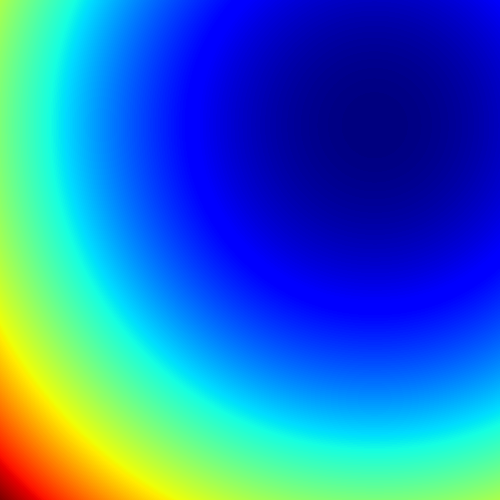
\includegraphics[width=0.8\linewidth]{forcing.png}
     \end{center}
     \captionof{figure}{Forcing function}
     \label{fig:forcing}
  \end{Figure}

  \begin{Figure}
     \begin{center}
       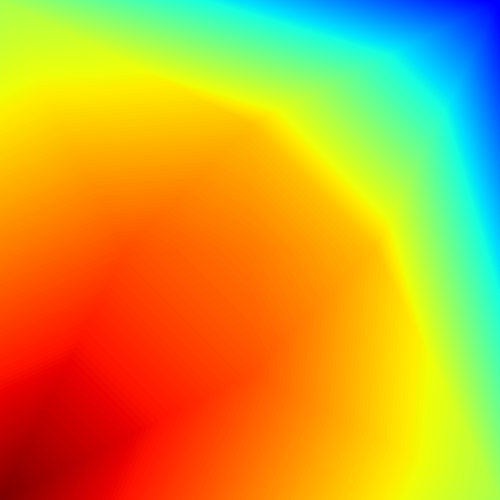
\includegraphics[width=0.8\linewidth]{CASE_2.png}
     \end{center}
     \captionof{figure}{CASE2 approximation with specified boundary conditions}
     \label{fig:CASE_2}
  \end{Figure}
\end{multicols}

\begin{multicols}{2}
  \begin{Figure}
     \begin{center}
       
\includegraphics[width=0.8\linewidth]{CASE_1.png}
     \end{center}
     \captionof{figure}{CASE1 approximation with boundary conditions of $0$}
     \label{fig:CASE_1}
  \end{Figure}

  \begin{Figure}
     \begin{center}
       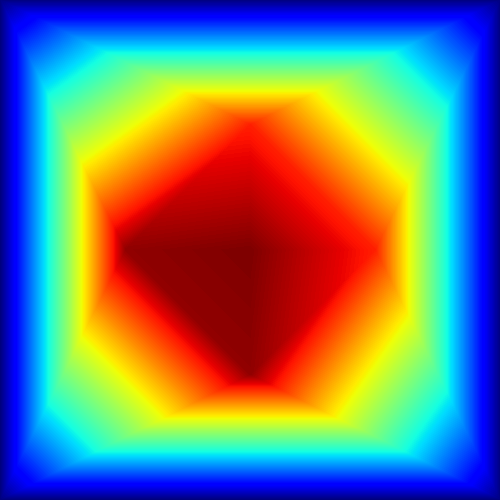
\includegraphics[width=0.8\linewidth]{CASE_1b.png}
     \end{center}
     \captionof{figure}{CASE1 approximation with boundary conditions of $0$, but
     with automatic color range.}
     \label{fig:CASE_1b}
  \end{Figure}
\end{multicols}

I just want to note that CASE2 looks weird. I'm hopeful that this is just due
the grain size of the mesh, but I also think that a better solution would be if
it were rotated by $180^\circ$, then inverse the colors. I am fearful that it
looks strange because of the C++ plotting that I have setup, so I need to do
some more checking of that process. But CASE1 looks pretty good, Its clear that
the part in the upper right is indeed lower, and the bottom left is the
maximum, but then everything stays relatively close to zero, because of the
boundaries.

I've also added a plot of my proposed "better" approximation for case 2.

\begin{Figure}
   \begin{center}
     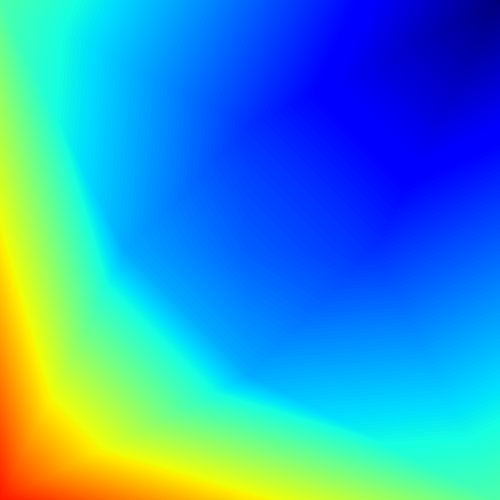
\includegraphics[width=0.5\linewidth]{CASE_2b.png}
   \end{center}
   \captionof{figure}{A possible better approximation, which is not what is
   found by the computer???}
   \label{fig:CASE_2b}
\end{Figure}

This was just an initial pass by hand, I have not rigorously verified that all
of my algorithms work as intended. So I still need to do more testing for my
integration and derivatives algorithms, to make sure that they are not the
source of the issue.

One thing is very clear though. THIS IS NOT A PROCESS MEANT FOR HUMANS. It's
terrible to do all of this by hand, It is very much meant for computers, but it
was good to do it by hand, as some of the matrix assembly make a lot more
sense.

\end{document}
